\documentclass[border=3pt,tikz]{standalone}
\usepackage{amsmath}
\usetikzlibrary{calc}
\usetikzlibrary{arrows.meta} % for arrow size
\begin{document}
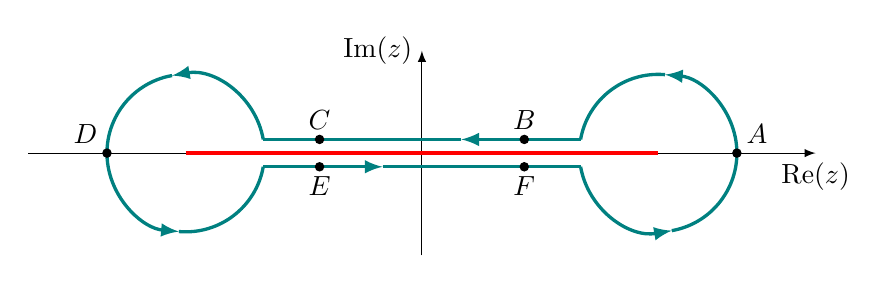
\begin{tikzpicture}[scale=1]
    \usetikzlibrary {arrows.meta}
    \usetikzlibrary {calc}
    
    \draw [-latex] (-5, 0) -- (5, 0) node[below] {Re$(z)$};
    \draw [-latex] (0, -1.3) -- (0, 1.3) node[left] {Im$(z)$};
    
    \draw[teal, very thick, -latex,] ({3+cos(190)}, {sin(190)}) arc (190:280:1);
    \draw[teal, very thick, -latex] ({3+cos(280)}, {sin(280)}) arc (280:445:1);
    \draw[teal, very thick] ({3+cos(85)}, {sin(85)}) arc (85:170:1);
    
    \draw[teal, very thick, -latex] ({3+cos(170)}, {sin(170)}) -- (0.5, {sin(170)});
    \draw[teal, very thick,] (0.5, {sin(170)}) -- ( {-3+cos(10)}, {sin(170)});
    
    \draw[teal, very thick, -latex,] ({-3+cos(10)}, {sin(10)}) arc (10:100:1);
    \draw[teal, very thick, -latex,] ({-3+cos(100)}, {sin(100)}) arc (100:265:1);
    \draw[teal, very thick,] ({-3+cos(265)}, {sin(265)}) arc (265:350:1);
    
    \draw[teal, very thick, -latex] ({-3+cos(350)}, {sin(350)}) -- (-0.5, {sin(350)});
    \draw[teal, very thick,] (-0.5, {sin(350)})-- ({3+cos(190)}, {sin(190)});
    
    \draw[red, very thick] (-3, 0) -- (3, 0);
    
    \filldraw [] (4,0) circle (1.5pt) node [above right] {$A$} ;
    \filldraw [] (1.3, {sin(170)}) circle (1.5pt) node[above] {$B$};
    \filldraw [] (-1.3, {sin(170)}) circle (1.5pt) node[above] {$C$};
    \filldraw [] (-4,0) circle (1.5pt) node [above left] {$D$} ;
    \filldraw [] (-1.3, {-sin(170)}) circle (1.5pt) node[below] {$E$};
    \filldraw [] (1.3, {-sin(170)}) circle (1.5pt) node[below] {$F$};
    \end{tikzpicture}
\end{document}